\documentclass[11pt]{beamer}
\usepackage[utf8]{inputenc}
\usepackage[russian]{babel}
\usepackage{multicol}
\usepackage{graphicx}
\usepackage{color}
\usepackage{colortbl}

\begin{document}

\begin{frame}{
\includegraphics[scale=0.3]{Logo.jpg}Перевод из одной СС в другую. Пример 1}
\begin{center}
    
$231_{(10)}=ABC_{(10)}=...HGFE_{(8)}=...+H*8^3+G*8^2+F*8+E$, при натуральных \textit{H,G,F,E} < 8.
$$\textcolor{green}{\textbf{Как найти \textit{E,F,G,H?}}}$$
Решение:$(...+H*8^3+G*8^2+F*8+E)/8=...+H*8^2+G*8^1+F$ (плюс остаток \emph{E}) => $(...HGFE_{(8)})/8=...HGF_{(8)} (с остатком E)$\vspace{0.2cm}
\begin{tabular}{%
|>{\color{white}\columncolor{black}}l|c|c|c|c|c|c|}
\hline
Номер шага \textit{(i)} & 0 & 1 & 2 & 3 & 4 & ...\\
\hline
Частное от деления на 8 & 231 & 28 & 3 & 0 & 0 & 0\\
\hline
Остаток от деления на 8 & 0 & 7 & 4 & 3 & 0 & 0\\
\hline
\end{tabular}
\\
\vspace{0.3cm}
\textcolor{green}{\textbf{Ответ}}: \emph{E}=7,\emph{F}=4,\emph{G}=3, \emph{H}=0.\\
$231_{(10)}=347_{(8)}$
\end{center}
\end{frame}

\begin{frame}{
\includegraphics[scale=0.3]{Logo.jpg}Перевод из одной СС в другую. Пример 2}
\begin{minipage}{0.4\textwidth}
\textbf{\Large Задача}: $231_{(10)}=?_{(2)}$
\vspace{1cm}\newline

\raggedleft\textbf{Ход решения $\rightarrow$}

\vspace{1cm}\newline
\raggedright\textbf{Ответ}: $231_{(10)}=11100111_{(2)}$
\end{minipage}
\hfill
\begin{minipage}{0.55\textwidth}
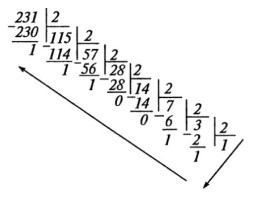
\includegraphics[scale=0.7]{frac.jpg}
\end{minipage}
\end{frame}

\begin{frame}{
\includegraphics[scale=0.3]{Logo.jpg}Перевод из одной СС в другую. Пример 2}
\begin{minipage}{0.5\textwidth}
\textbf{Задача}: $0,8125_{(10)}=?_{(2)}$

\vspace{1cm}

\textbf{Ход решения \rightarrow}
\end{minipage}
\hfill
\begin{minipage}{0.45\textwidth}
\begin{tabular}{|c|c|}
     \hline
     0 & ,8125\\
       & 2\\
    \hline
    \textcolor{red}{1} & ,625\\
       & 2\\
    \hline
    \textcolor{red}{1} & ,25\\
       & 2\\
    \hline
    \textcolor{red}{0} & ,5\\
       & 2\\
    \hline
    \textcolor{red}{1} & 0\\
    \hline
\end{tabular}
\end{minipage}
\vspace{0.6cm}

\textbf{Ответ}: $0,8125_{(10)}=1*2^{-1}+1*2^{-2}+1*2^{-4}=0,1101_{(2)}$
\end{frame}

\begin{frame}{
\includegraphics[scale=0.3]{Logo.jpg}Преобразование из \emph{CC}-\emph{N} в $CC-N^k$ и обратно}
\textbf{\textcolor{green}{Из $CC-N$ в $CC-N^k$}}
\begin{itemize}
    \item дополнить число, записанное в СС с основанием \emph{N}, незначащими нулями так, чтобы количество цифр было кратно \emph{k};
    \item разбить полученное число на группы по \emph{k} цифр, начиная от нуля;
    \item заменить каждую такую группу эквивалентным числом, записанным в СС с основанием $N^k$.
\end{itemize}\newline
\qquad\qquadЗадача: $1020101_{(3)}=?_{(5)}$\\
\qquad\qquadРешение: $1020101_{(3)}=001020101_{(3)}=16A?_{(27)}$

\textbf{\textcolor{green}{Из $CC-N^k$ в $CC-N$}}
\begin{itemize}
    \item заменить каждую цифру числа, записанного в CC с основанием $N^k$, эквивалентным набором из \emph{k} цифр CC с основанием \emph{N}.
\end{itemize}
\qquad\qquadЗадача: $2345_{(125)}=?_{(5)}$\\
\qquad\qquadРешение: $2345_{(125)}=002003004010_{(5)}=2003004010_{(5)}$
\end{frame}

\begin{frame}{
\includegraphics[scale=0.3]{Logo.jpg}Оптимальная система счисления}
\textbf{Задача}. Робинзон Крузо нашёл на острове 60 камней. Сколько прошедших дней можно ими закодировать в разных СС?
\vspace{0.8cm}

\begin{minipage}{0.27\textwidth}
\textbf{Пример СС-10}:
\end{minipage}
\begin{minipage}{0.25\textwidth}

\includegraphics[scale=0.5]{graphic.jpg}
\end{minipage}
\begin{minipage}{0.45\textwidth}
463502-й день из 999999 возможных, где 999999=$10^6-1$
\begin{center}
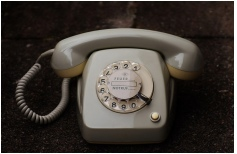
\includegraphics[scale=0.48]{phone.jpg}
\end{center}
\end{minipage}
\hfill
\end{frame}

\begin{frame}{
\includegraphics[scale=0.3]{Logo.jpg}Оптимальная система счисления(2)}

\begin{minipage}{0.4\textwidth}
\textbf{Пример СС-60}:\\
\newline
0 камней = 0 дней\\
1 камень = 1 день\\
2 камня = 2 дня\\
...\\
\textbf{60 камней} = 60 дней
\end{minipage}
\hfill
\begin{minipage}{0.3\textwidth}
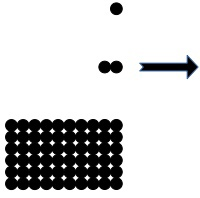
\includegraphics[scale=0.4]{balls.jpg}
\end{minipage}
\hfill
\begin{minipage}{0.25\textwidth}
1 день\\
\newline
2 дня\\

\vspace{0.2cm}
60 дней
\vspace{0.5cm}
\end{minipage}
\end{frame}
\end{document}